\documentclass{beamer}
\usepackage{amsmath}
\usepackage{graphicx}
\usepackage{subfigure}

%\usepackage{caption}
%\usepackage{subcaption}

% Copyright 2004 by Till Tantau <tantau@users.sourceforge.net>.
%
% In principle, this file can be redistributed and/or modified under
% the terms of the GNU Public License, version 2.
%
% However, this file is supposed to be a template to be modified
% for your own needs. For this reason, if you use this file as a
% template and not specifically distribute it as part of a another
% package/program, I grant the extra permission to freely copy and
% modify this file as you see fit and even to delete this copyright
% notice. 


\mode<presentation>
{
  \usetheme{default}
  % or ...

  \setbeamercovered{transparent}
  % or whatever (possibly just delete it)
}


\usepackage[english]{babel}
% or whatever

\usepackage[utf8]{inputenc}
% or whatever

\usepackage{xcolor}
\usepackage[percent]{overpic}

\usefonttheme{serif}
\usecolortheme{seahorse}

\usepackage[T1]{fontenc}

\title[April APS]
{Active Resonators for ADMX}

\author[Malagon]
{Ana Malag\'on}

\institute[University of Washington]
{University of Washington, ADMX Collaboration}

\date[April 15, 2015]
{April 15, 2015 / April APS Meeting}

\begin{document}

\begin{frame}
\titlepage
\end{frame}

\begin{frame}{Idea}
\begin{itemize}
\item Axion microwave cavity haloscopes use microwave cavities.

\item Expected signal power is proportional to Q:
\begin{align*}
P_{sig} \propto \text{min}\big(Q_L, Q_a\big)
\end{align*}
axion quality factor: $Q_a \simeq 10^6$
\item Theoretical Q goes as 
\begin{align*}
Q = \frac{L}{R+L}\frac{R}{\delta}
\end{align*}

\item anomalous skin depth (Cu): $\delta = 2.8\times10^{-5}\text{ cm}\bigg(\frac{\text{GHz}}{f}\bigg)^{1/3}$

\item  $Q_L \approx 10^5$ for $f \approx 1$ GHz.


\item Can we increase the loaded Q further? 
\end{itemize}
\end{frame}

\begin{frame}{Active Feedback}
\centering
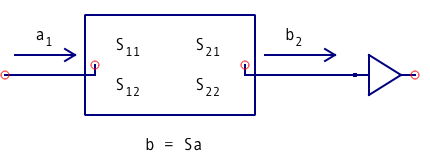
\includegraphics[width=0.6\textwidth]{export_sparams_10}
\end{frame}

\begin{frame}{Active Feedback}
\centering
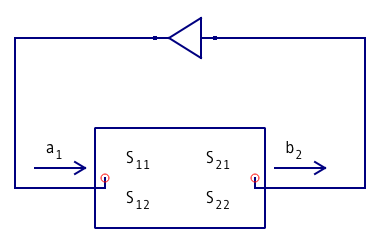
\includegraphics[width=0.65\textwidth]{export_sparams_4}
\end{frame}

\begin{frame}{Active Feedback}
\centering
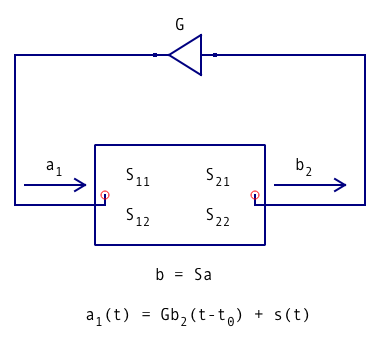
\includegraphics[width=0.65\textwidth]{export_sparams_7}
\end{frame}

\begin{frame}{Active Feedback}
\centering
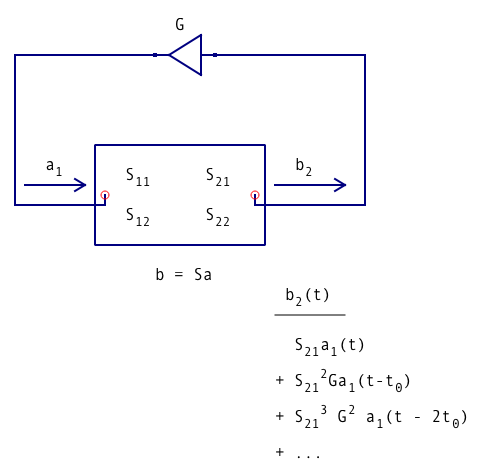
\includegraphics[width=0.65\textwidth]{export_sparams_8}
\end{frame}

\begin{frame}{Active Feedback}
\centering
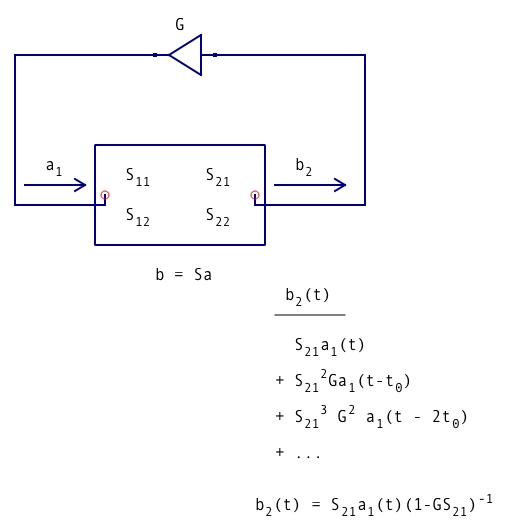
\includegraphics[width=0.65\textwidth]{export_sparams_9}
\end{frame}


\begin{frame}{Active Feedback}
\centering
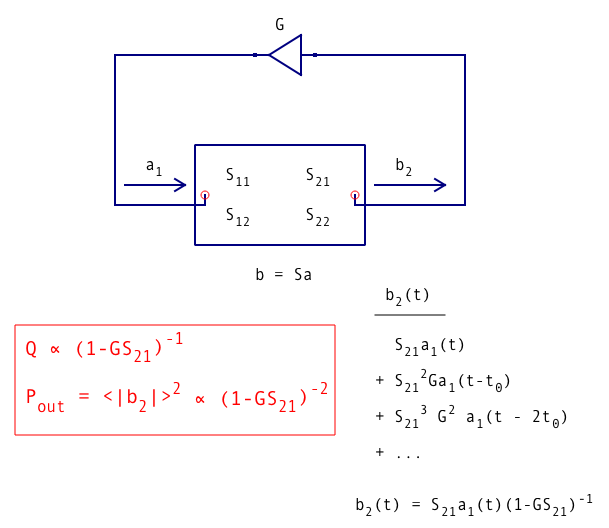
\includegraphics[width=0.65\textwidth]{export_sparams_13}
\end{frame}

\begin{frame}{Active Feedback}
\centering
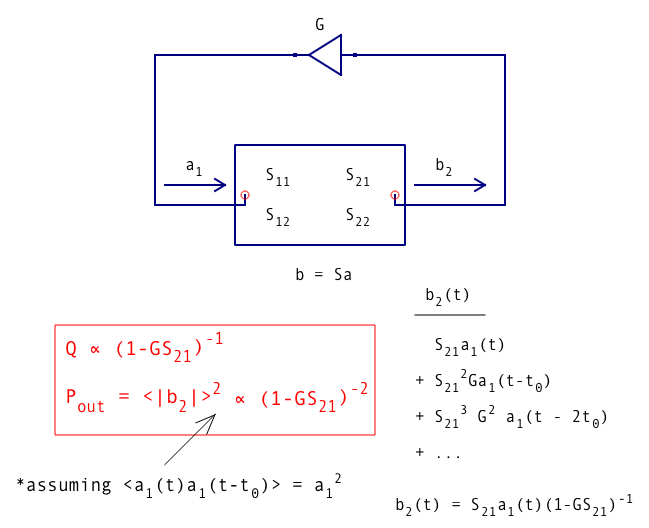
\includegraphics[width=0.65\textwidth]{export_sparams_14}
\end{frame}

\begin{frame}
\begin{itemize}
\item This idea is old; patented in 1914 and used for making higher gain amplifiers and more selective radio circuits. 

\item However, this amplifies noise and signal equally, so SNR should remain constant$^{*}$.

\item ${^*}$Since axion signal goes with $Q$, SNR increases
\begin{align*}
\text{SNR}_{\text{axion}} \propto (1-x)^{-1}
\end{align*}
\item We can utilize the different coherence times of signal and noise to get more improvement.
\end{itemize}
\end{frame}

\begin{frame}{Noise}
\centering
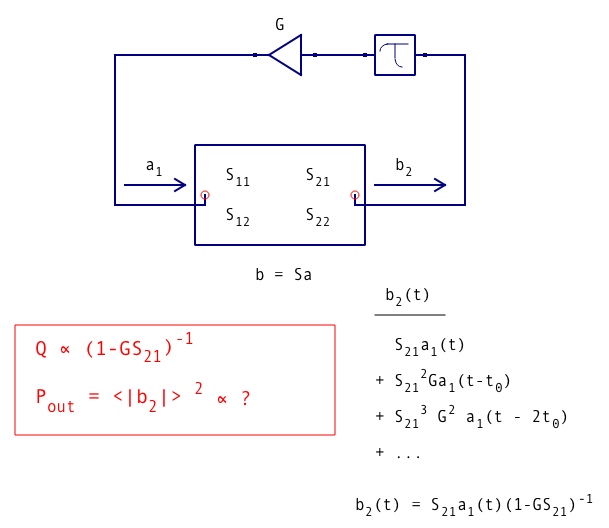
\includegraphics[width=0.6\textwidth]{export_sparams_12}
\end{frame}

\begin{frame}{Active Feedback Resonator}
{\tiny Ouroboros}
%\begin{columns}
%\column{0.5\textwidth}
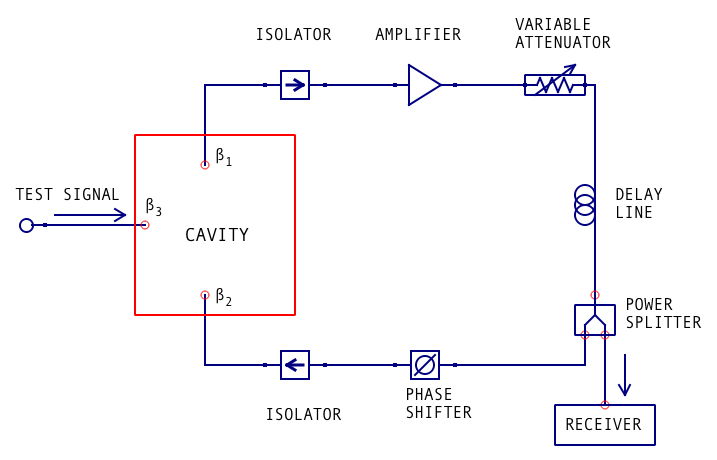
\includegraphics[width=\textwidth]{export_ouroboros}
%\column{0.5\textwidth}
%\begin{itemize}
%\item $t$: time around loop
%\item $\tau$: coherence time of cavity
%\item Intuition: signal feeds back coherently; when $t > \tau$, noise adds incoherently
%\end{itemize}
%\end{columns}
\end{frame}

\begin{frame}{Parameters}
delay time: 2.4 $\mu$seconds

$Q \simeq 1200$

$f = 2.256$ GHz
\end{frame}


\begin{frame}{People}
\begin{columns}
\column{0.5\textwidth}
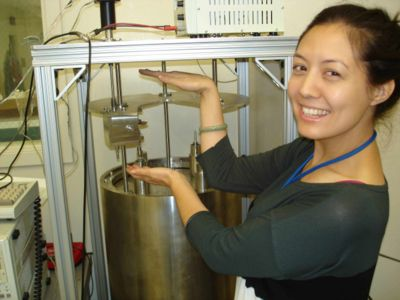
\includegraphics[width=0.8\textwidth]{lisa_pic}
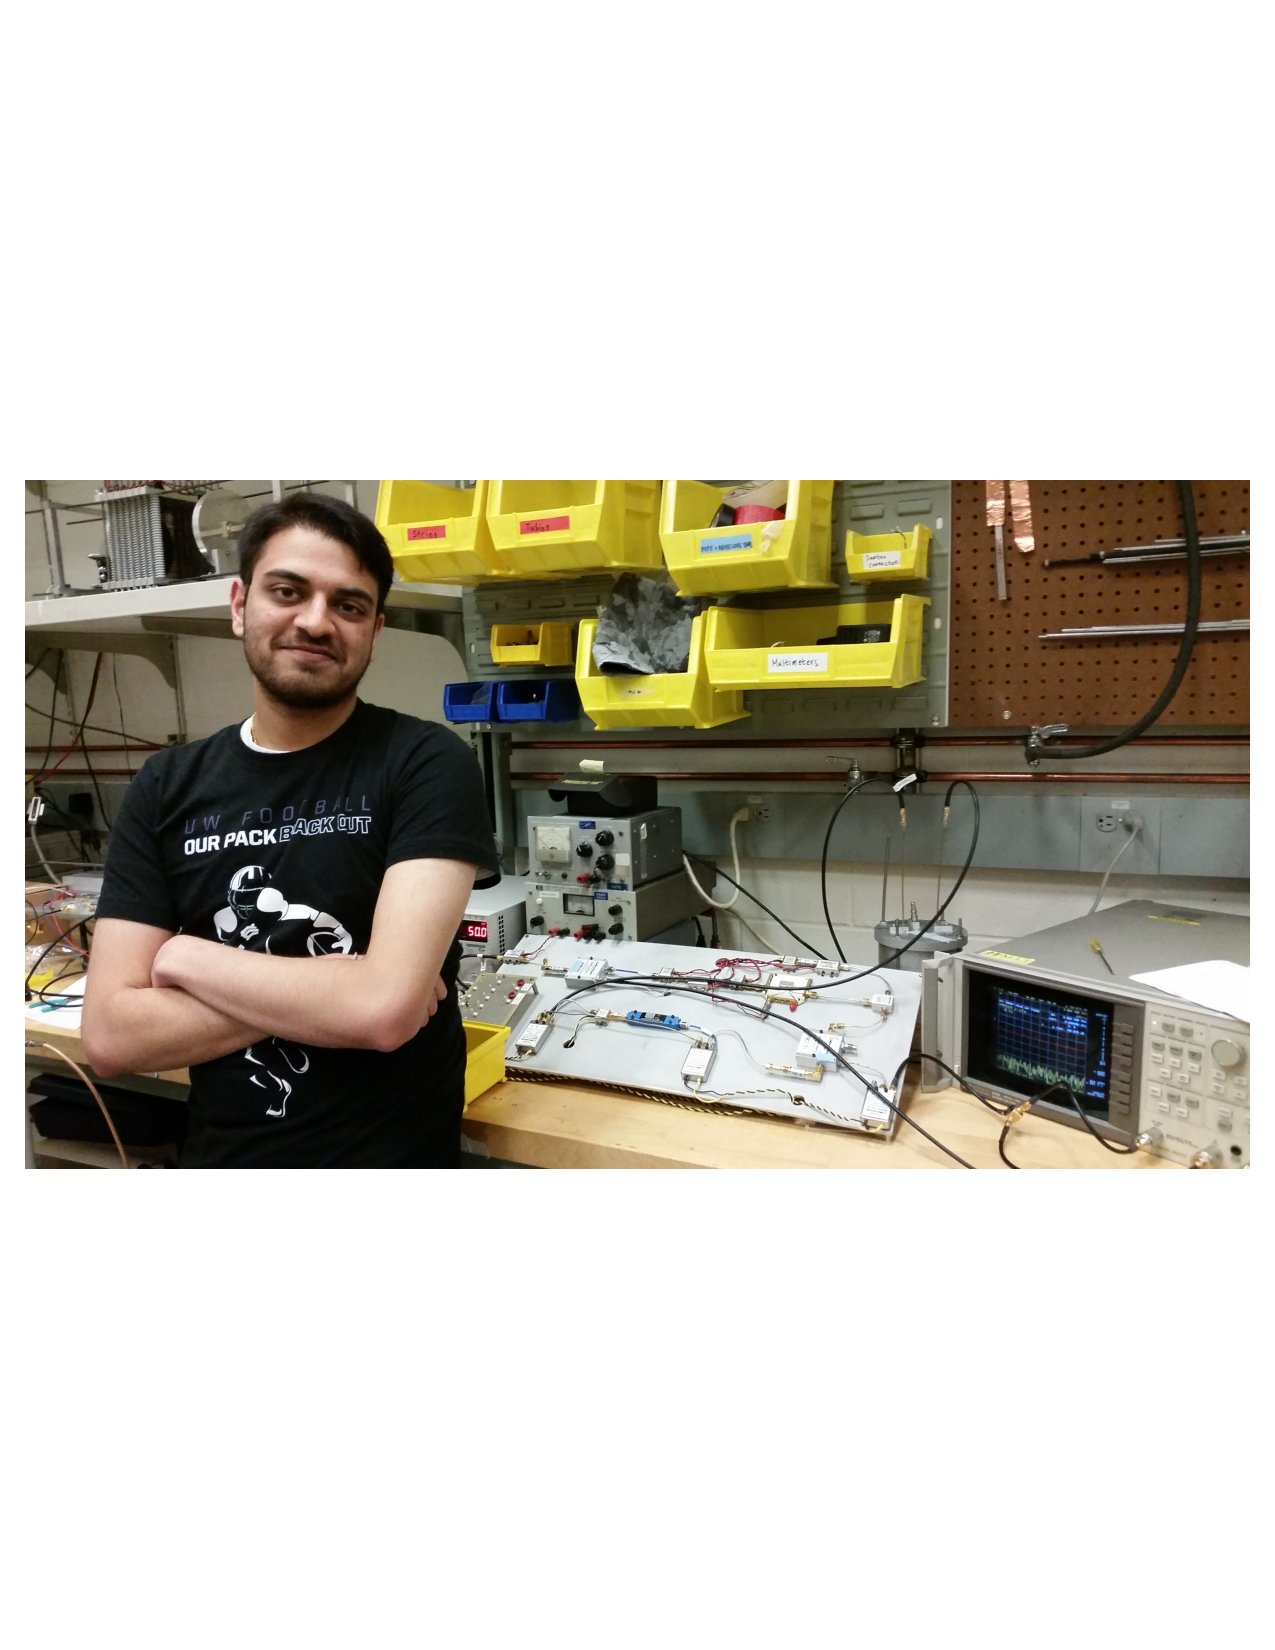
\includegraphics[width=\textwidth]{kunal_pic}

\column{0.5\textwidth}
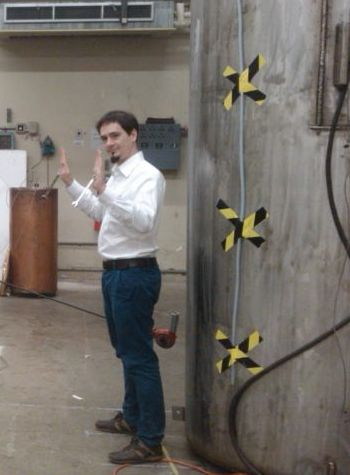
\includegraphics[width=\textwidth]{gray_pic}

\end{columns}
\end{frame}

\begin{frame}{Axion and CW Signal}
{\tiny Scenario 1}
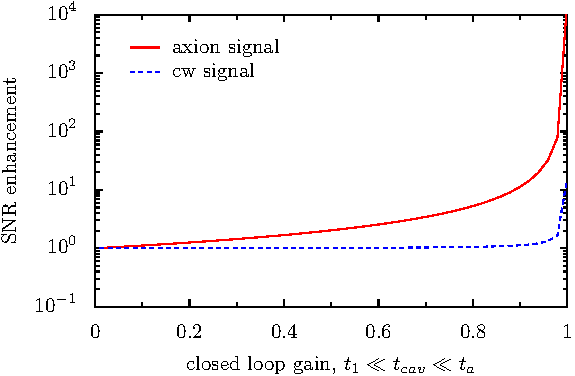
\includegraphics[width=\textwidth]{first_limit}

\end{frame}

\begin{frame}{Axion and CW Signal}
{\tiny Scenario 2}
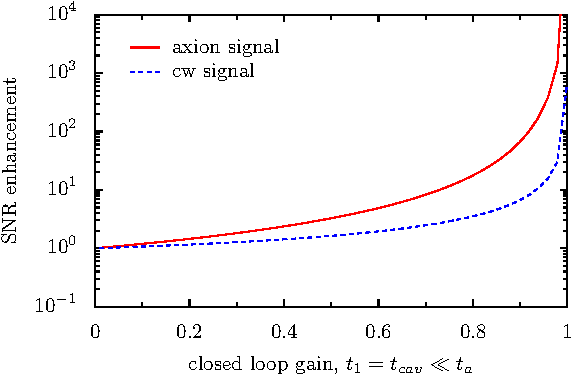
\includegraphics[width=\textwidth]{second_limit}
\end{frame}

\begin{frame}{Axion and CW Signal}
{\tiny Scenario 3}
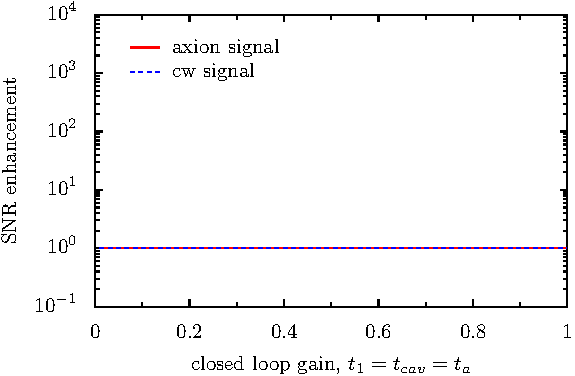
\includegraphics[width=\textwidth]{third_limit}
\end{frame}

\begin{frame}{Exploring Second Limit}
{\tiny$t_1 \ll t_{cav}$}
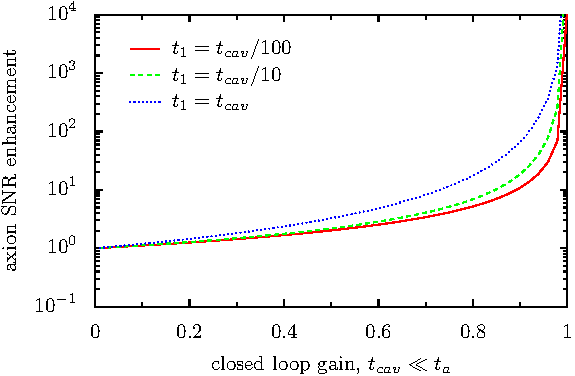
\includegraphics[width=\textwidth]{exploring_second_limit_low}
\end{frame}

\begin{frame}{Exploring Second Limit}
{\tiny $t_1 > t_{cav}$}
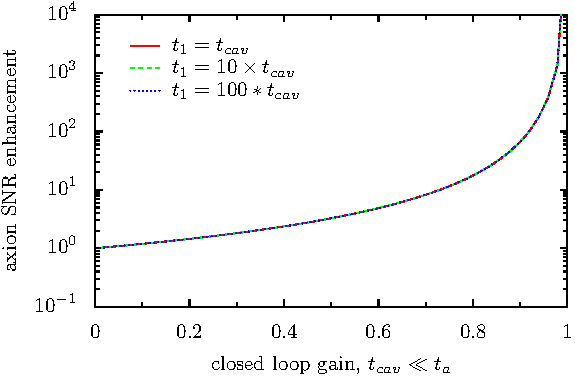
\includegraphics[width=\textwidth]{exploring_second_limit_high}
\end{frame}

\begin{frame}{Theory and Experiment}
{Comparison}
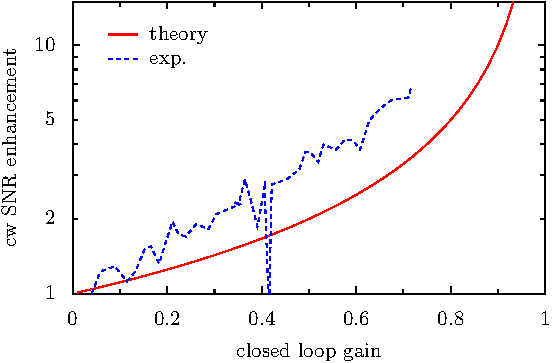
\includegraphics[width=\textwidth]{comparison_xaxis_gain}
\end{frame}


\begin{frame}{Active Feedback Resonator}
{\tiny Ouroboros}
\begin{columns}
\column{0.5\textwidth}
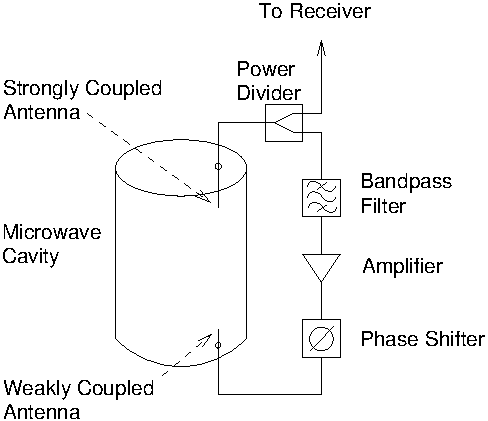
\includegraphics[width=\textwidth]{experiment_schematic-eps-converted-to}
\column{0.5\textwidth}
\begin{itemize}
\item $t$: time around loop
\item $\tau$: coherence time of cavity
\item Intuition: signal feeds back coherently; when $t > \tau$, noise adds incoherently
\end{itemize}
\end{columns}
\end{frame}

\begin{frame}{Equivalent Circuit}
\centering
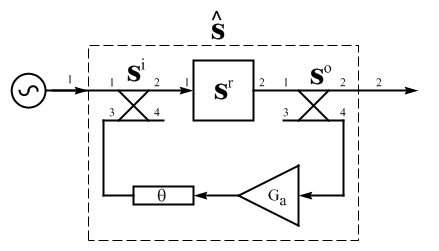
\includegraphics[width=.5\textwidth]{qmultiplier}

$G_l$ the loop gain\\
$Q_0$ the active quality factor\\
$T_a$ the amplifier noise temperature\\
%$T_{cav}$ the cavity noise temperature\\
\begin{columns}
\column{0.5\textwidth}
\centering
\begin{align*}
Q_0 = Q_L(1-\sqrt{G_l})^{-1} \\
|\hat{S}_{21}|^2 \propto (1- \sqrt{G_l})^{-2}
\end{align*}
\column{0.5\textwidth}
\centering
\begin{align*}
T_{noise} = \frac{T_{cav} + G_l T_a}{1 + G_l - 2\sqrt{G_l}e^{-t/\tau - i\theta}}
\end{align*}
\end{columns}
\end{frame}

\begin{frame}{Prototype}
\begin{columns}
\column{0.5\textwidth}
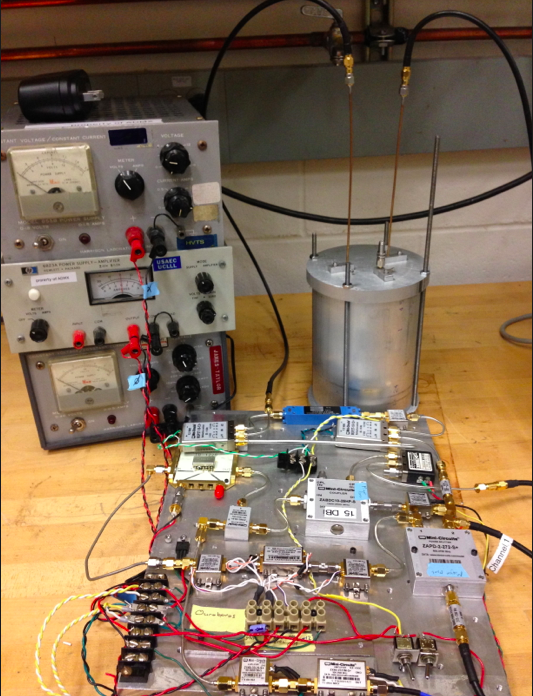
\includegraphics[width=\textwidth]{active_resonator_setup_photo}
\column{0.5\textwidth}
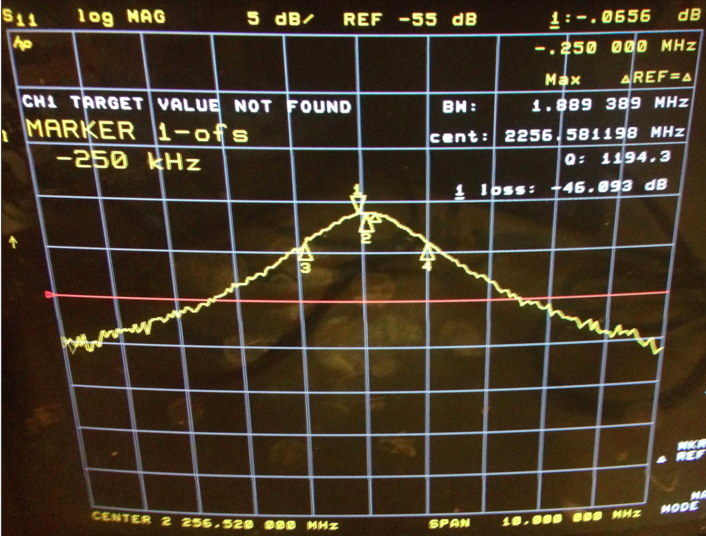
\includegraphics[width=\textwidth]{s21_no_delay}

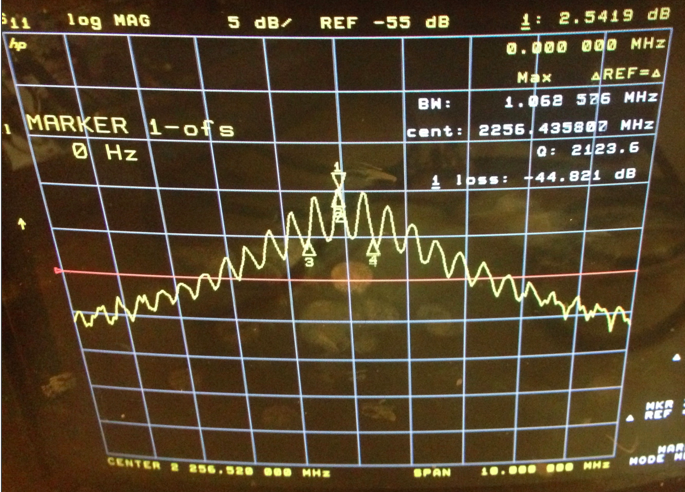
\includegraphics[width=\textwidth]{s21_delay}
\end{columns}

\end{frame}

\begin{frame}{Results}
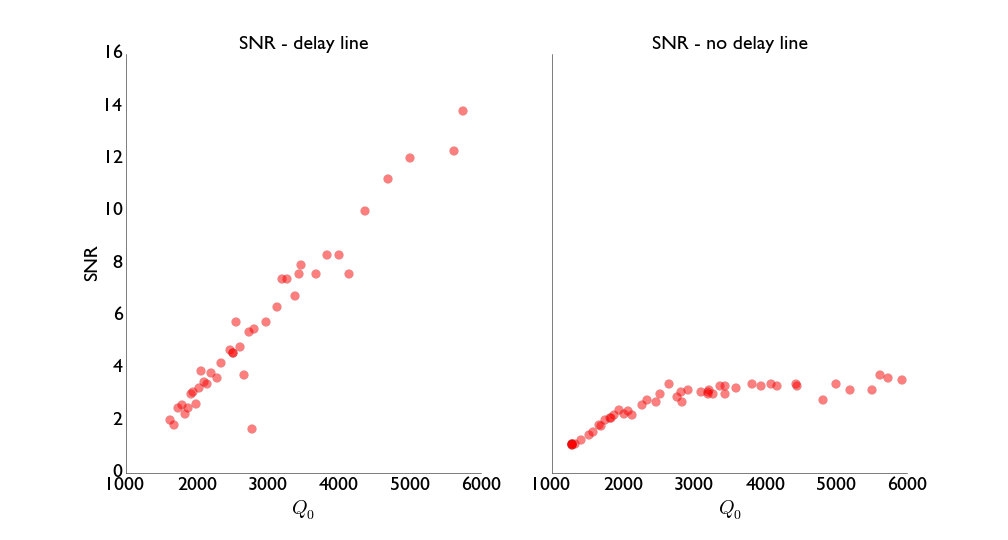
\includegraphics[width=\textwidth]{summary_plots}
\end{frame}

\begin{frame}{Acknowledgments}
DOE HEP
\end{frame}

\end{document}